% ================================
% Research Question and Case Justification
% ================================

\section*{Research Question and Case Justification}
\addcontentsline{toc}{section}{Research Question and Case Justification}

Actors are classified into four types used consistently across hypotheses, 
tables, and coding: 
\begin{enumerate}
  \item State agencies and intergovernmental bodies
  \item NGOs and civil society organizations
  \item Business associations and industry groups
  \item Scientific and academic institutions
\end{enumerate}

\subsection*{Research Question}

\begin{quote}
\textbf{Under what institutional conditions do actors engage in ideational
bricolage in forest adaptation governance, and how does this shape the uptake
of their ideas across policy arenas?}
\end{quote}

\textbf{Hypotheses:}  
\begin{enumerate}
    \item \textbf{H1 (Institutional Density).} In high-density systems
    (Germany), bricolage will primarily take the form of layering, producing
    higher average Uptake Index scores across venues.
    \item \textbf{H2 (Institutional Fragmentation).} In fragmented systems
    (Chile), bricolage will favor transposition and recombination, producing
    uptake concentrated in fewer venues but with higher variance.
    \item \textbf{H3 (Actor Type).} State actors will achieve higher Uptake
    Index scores than NGOs and civil society organizations, business
    associations, or scientific and academic institutions. The gap will be
    narrower in Chile due to reliance on civil society and academic expertise.
\end{enumerate}

\subsection*{Testing Strategy}

\textbf{H1 (Density).} Compare Uptake Index distributions between Germany and
Chile using descriptive statistics (medians, interquartile ranges) and visual
comparisons (boxplots, density plots).  

\textbf{H2 (Fragmentation).} Assess variance descriptively by reporting spread
measures (range, IQR) and distributional shapes across the two cases.  

\textbf{H3 (Actor Type).} Within each country, compare Uptake Index scores
across actor types by reporting group medians, ranges, and graphical displays.
Cross-tabulations (e.g., high vs. low uptake categories by actor type) will be
used to illustrate differences.  

The emphasis is on \textbf{patterns, contrasts, and substantive meaning}, not
statistical significance. The objective is to assess whether observed
differences are consistent with theoretical expectations.

Discursive institutionalism specifies coordinative and communicative modes of
discourse, while bricolage highlights how actors recombine elements of
institutional toolkits. The integration is causal: discourse frames (diagnostic,
prognostic, motivational) inform the selection and recombination of instruments,
which in turn generate uptake pathways. Figure~\ref{fig:causal} maps this chain
and directly grounds Hypotheses H1–H3.

\begin{figure}[h!]
  \centering
  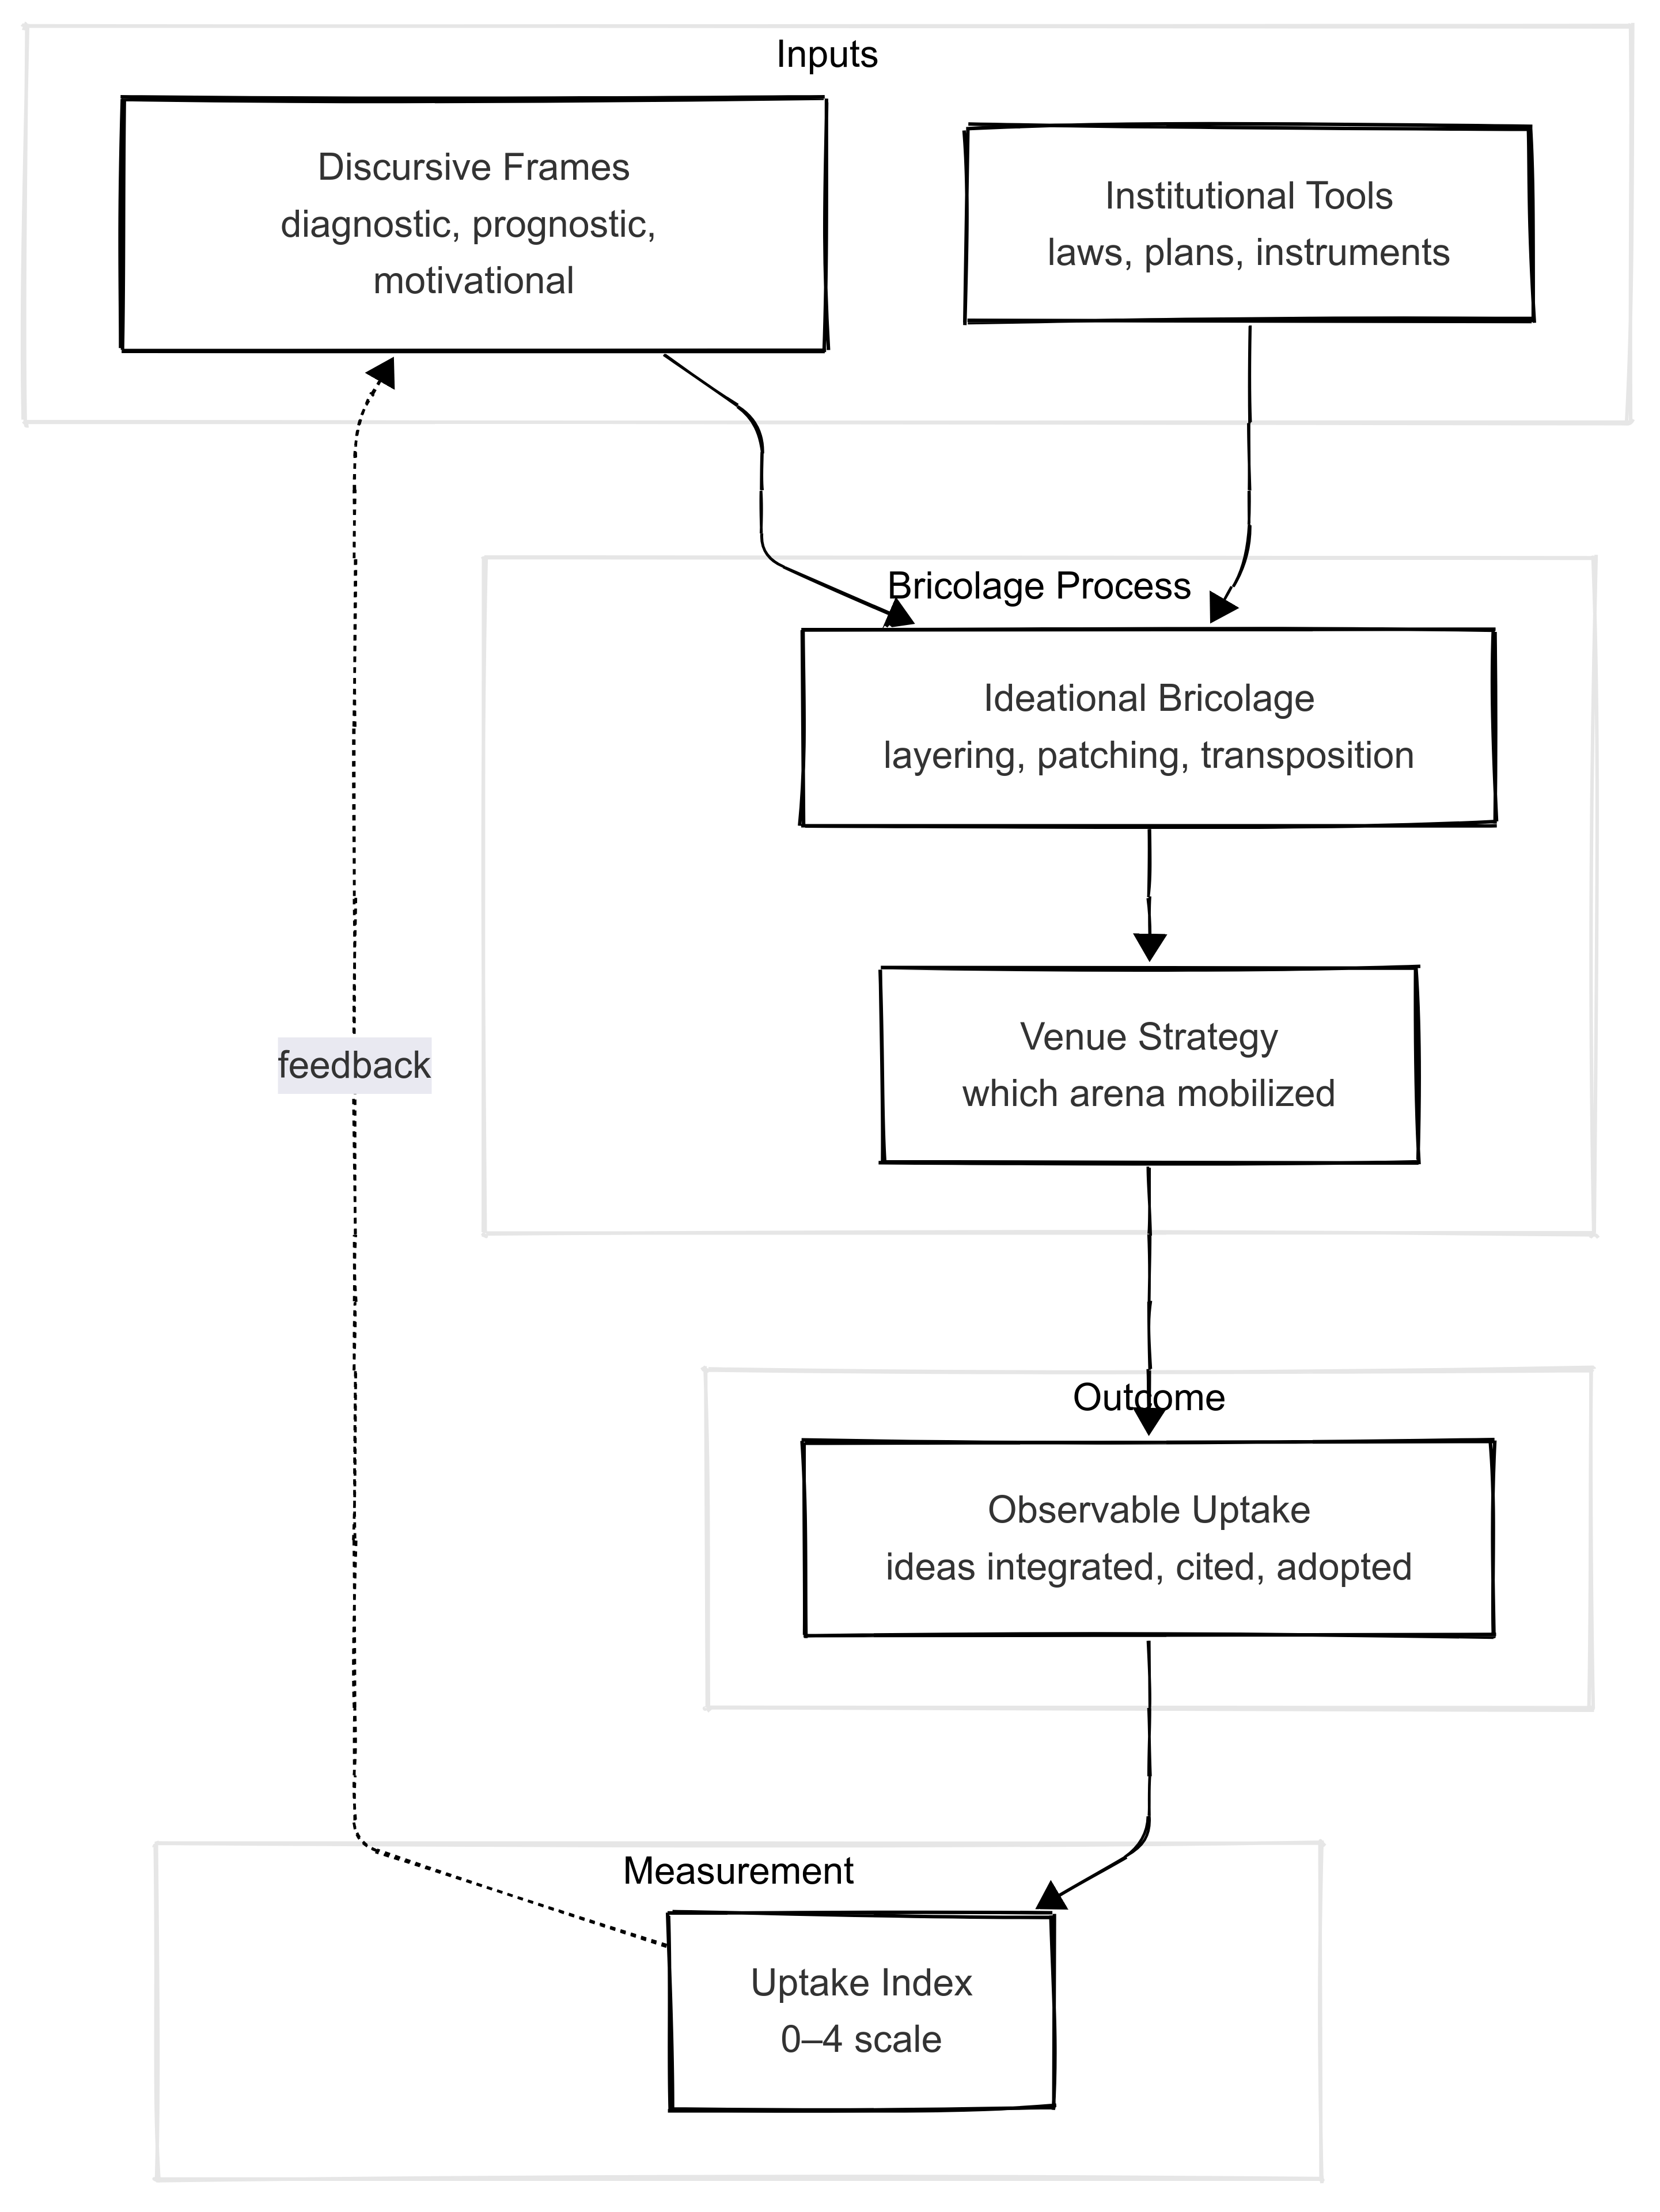
\includegraphics[width=0.8\textwidth]{src/fig/prop/03/modal.pdf}
    \caption{Causal model linking discursive institutionalism and ideational
    bricolage. Discourse frames feed into bricolage modes (layering, patching,
    transposition). Institutional context (density, fragmentation, veto points)
    conditions these processes. Actor type moderates uptake pathways, which are
    observed through text reuse, funding allocations, institutional incorporation, 
    and representation in decision-making venues.}
\label{fig:causal}
\end{figure}

As shown in Figure~\ref{fig:causal}, the causal chain links discourse frames 
to bricolage modes, which then translate into observable uptake.  

H1 derives from institutional density: in dense systems, layering is more 
feasible, leading to gradual but consistent uptake across multiple venues.  

H2 follows from fragmentation: in weaker, incoherent systems, transposition and 
recombination dominate, producing uptake concentrated in few venues with greater 
variance.  

H3 follows from actor type: state actors generally achieve higher Uptake Index
scores than NGOs, business, or academic actors, although in Chile the gap
narrows because civil society and scientific institutions fill governance
capacity gaps.  

This framing shifts the inquiry from a descriptive catalogue of actors toward an 
explanatory design. The focus is on how institutional density, actor type, and
venue strategy condition the effectiveness of bricolage attempts. Effectiveness
is defined not by intent alone, but by \textbf{observable uptake in policy
processes}, such as text reuse in legislative drafts, allocation of pilot
funding, or inclusion in decision-making bodies.

\subsection*{Case Selection Justification}
Germany and Chile are selected as a \emph{most-different systems design} 
\parencite{George2005}. 
Both face analogous biophysical threats---severe droughts, wildfire 
regimes, and forest dieback---but are embedded in sharply contrasting 
political–institutional contexts. 
Germany represents a dense corporatist welfare state with strong 
consensus institutions, while Chile exemplifies a fragmented neoliberal 
system shaped by legacies of authoritarian reform and ongoing 
socio-environmental conflicts. 

Comparing these two maximizes analytical leverage: if similar bricolage 
strategies emerge under such divergent contexts, the explanatory value 
of the concept strengthens; if they diverge, the analysis clarifies how 
institutional logics shape adaptation governance.

\begin{table}[h!]
\centering
\caption{Comparative justification of case selection}
\begin{tabular}{@{}p{4cm}p{5cm}p{5cm}@{}}
\toprule
\textbf{Dimension} & \textbf{Germany} & \textbf{Chile} \\ \midrule
Biophysical stress (2010--2025) & Drought-induced tree mortality, bark beetle outbreaks; 4/5 trees diseased \parencite{BMEL2023} & Megadrought (2010--2020), catastrophic wildfires (2017, 2023) \\
Governance density & High: corporatist forestry councils, Länder–federal coordination, EU directives & Low: fragmented ministries, weak enforcement, dominance of private forestry firms \\
Forestry economy & Diversified multifunctional forestry, declining industrial share & Plantation-centered, export-driven (pine/eucalyptus), central to trade balance \\
Veto points & High: federalism, EU layering, corporatist negotiation arenas & Low: central executive dominance, weak checks, but strong social contestation \\
Key conflicts & Conservation vs. production discourses & Plantation model vs. indigenous/territorial rights discourses \\
Institutional legacy & Consensus corporatism, long-standing discursive struggles \parencite{Winkel2011} & Neoliberal reform legacy, privatized land/water regimes \parencite{Manuschevich2016} \\
\bottomrule
\end{tabular}
\end{table}

In sum, Germany offers a reference case of high-density institutional 
bricolage where layering and patching dominate, while Chile represents 
a fragmented context where transposition and novel assemblages are 
more likely. 
Their comparison avoids Eurocentric bias, foregrounds Global South 
perspectives, and enables a more generalizable understanding of 
ideational bricolage in adaptation governance.